\documentclass[aspectratio=169]{beamer}
\usepackage[utf8]{inputenc} % codificacao de caracteres
\usepackage[T1]{fontenc}    % codificacao de fontes
\usepackage[english]{babel}  % idioma
\usepackage{graphics,amssymb,amsfonts,amsmath}
\usepackage{tikz}
\usepackage{enumerate,hyperref}
\usepackage{palatino}	% Fonte sem serifa
\usepackage{ragged2e}	% Paragrafo justificado
%\usepackage{minted}	% Highlight para codigos de programacao
\usepackage{booktabs} % tabelas
\usepackage{multicol}
\usepackage{multirow}
%\usepackage[table]{xcolor}


% Veja mais temas e cores em http://www.hartwork.org/beamer-theme-matrix/
\usetheme{Montpellier}         % tema
\usecolortheme{orchid}      % cores
\usefonttheme[onlymath]{serif} % fonte modo matematico
% Colocando numero de paginas no slide
\setbeamertemplate{footline}[frame number]



\DeclareGraphicsExtensions{.pdf,.JPG,.png} % compilamos apenas com pdflatex
%\graphicspath{{./figuras/}} % caminho onde as figuras estarao disponiveis


\graphicspath{{figuras/}}

% ---------------------------------------------------------------------------- %
% T�tulo                                                                       %
% ---------------------------------------------------------------------------- %

\title[\sc{Teoria de Circuitos Eletrônicos 1}]{\LARGE Aula 5: Circuit Theorems}
\author[Prof. Marcelino Andrade]{Prof. Marcelino Andrade}
\institute{Faculdade UnB Gama} % opcional
\date{\today}

\begin{document}
\justifying % Paragrafo justificado
\pagebreak

\begin{frame}
  \titlepage
\end{frame}


% ----------------- NOVO SLIDE --------------------------------
\begin{frame}{Contents\newline}

\tableofcontents
\begin{center}	
     		Introduction to Electric Circuits 9th Edition by James A. Svoboda, Richard C. Dorf			
\end{center}	
\end{frame}

% ----------------- NOVA SECÇÂO -----------------------------
\section{Introduction (5.1)}
% ----------------- NOVO SLIDE --------------------------------
\begin{frame}[fragile]
	\frametitle{Introduction}
		\begin{tabular}{cc}
			\begin{columns}
				\begin{column}{1\textwidth}  %%<--- here
					In this chapter, we consider five circuit theorems:	\newline
		
					\begin{itemize}
						\item[$\clubsuit$]{Source Transformation;}
						\item[$\clubsuit$] {Superposition;}	
						\item[$\clubsuit$]{Thévenin's Theorem;}	
						\item[$\clubsuit$]{Norton’s Theorem;}	
						\item[$\clubsuit$]{The Maximum Power Transfer Theorem.\newline}				
					\end{itemize}
					
				\end{column}
			\end{columns}
		
	\end{tabular}
\end{frame}

% ----------------- NOVA SECÇÂO -----------------------------
\section{Source Transformations (5.2)}
% ----------------- NOVO SLIDE --------------------------------
\begin{frame}[fragile]
\frametitle{Source Transformations}
\begin{tabular}{r}
	\begin{columns}	\column{1\textwidth}
	The ideal voltage source is the simplest model of a voltage source, but occasionally we need a more
accurate model.
\newline
	\end{columns} \\
	\begin{columns}
		\begin{column}{0.5\textwidth}  %%<--- here
	%		\begin{center}
			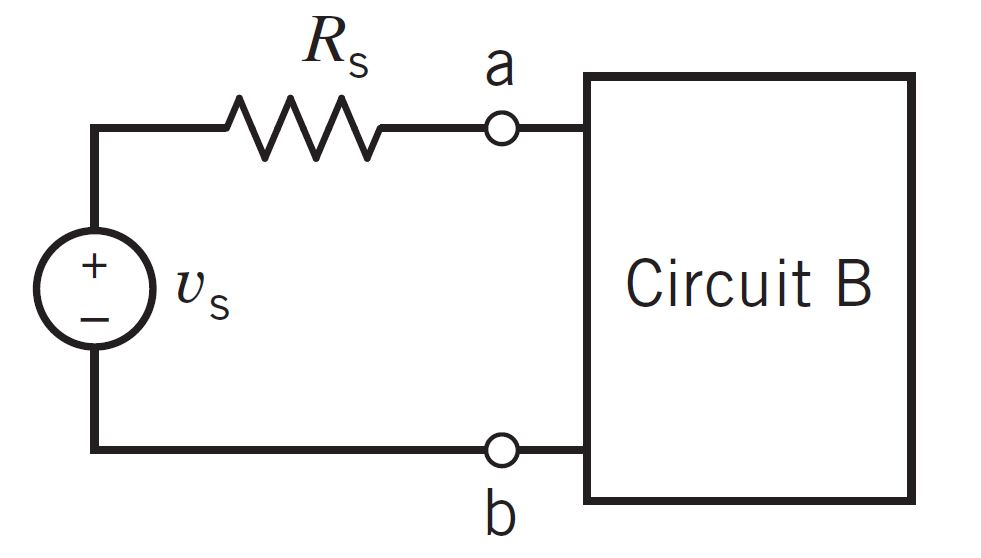
\includegraphics[height=3cm]{figura01.JPG}\\
			%	\end{center}			

		\end{column}
		\begin{column}{0.5\textwidth}  %%<--- here
			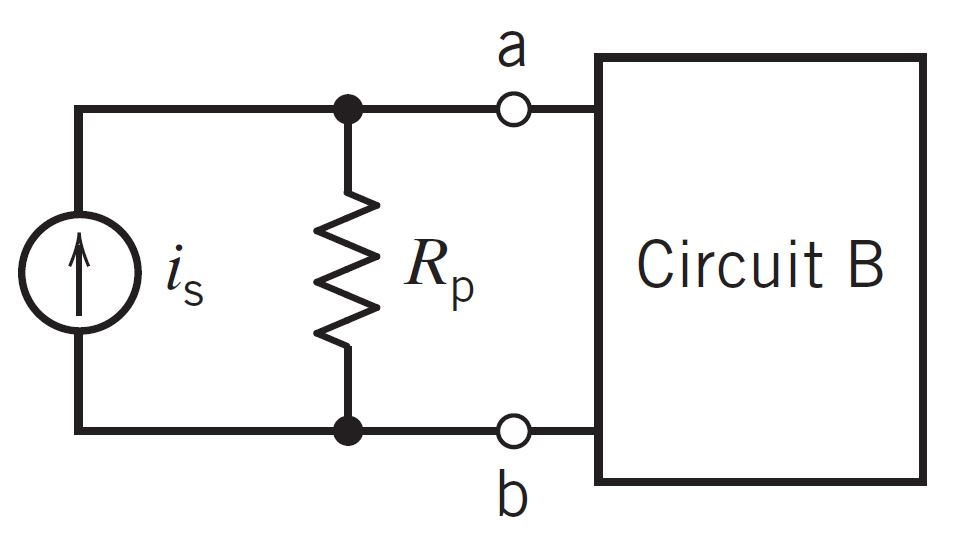
\includegraphics[height=3cm]{figura02.JPG}\\
		\end{column}
	\end{columns} \\

	\begin{columns}	\column{1\textwidth}
	\newline Under certain conditions $R_{p}=R_{s}$ and $v_{s}=R_{s}i_{s}$, the nonideal voltage source and the nonideal
current source are equivalent to each other.
	\end{columns}

\end{tabular}
\end{frame}
% ----------------- NOVO SLIDE --------------------------------
\begin{frame}[fragile]
\frametitle{Source Transformations}
\begin{tabular}{r}
	\begin{columns}	\column{1\textwidth}
	We connect a resistor having resistance $R$ to the terminals of the test circuit and measure the resistor voltage $v$ and resistor current $i$. 
\newline
	\end{columns} \\
	\begin{columns}
		\begin{column}{0.33\textwidth}  %%<--- here
		%	\begin{center}
			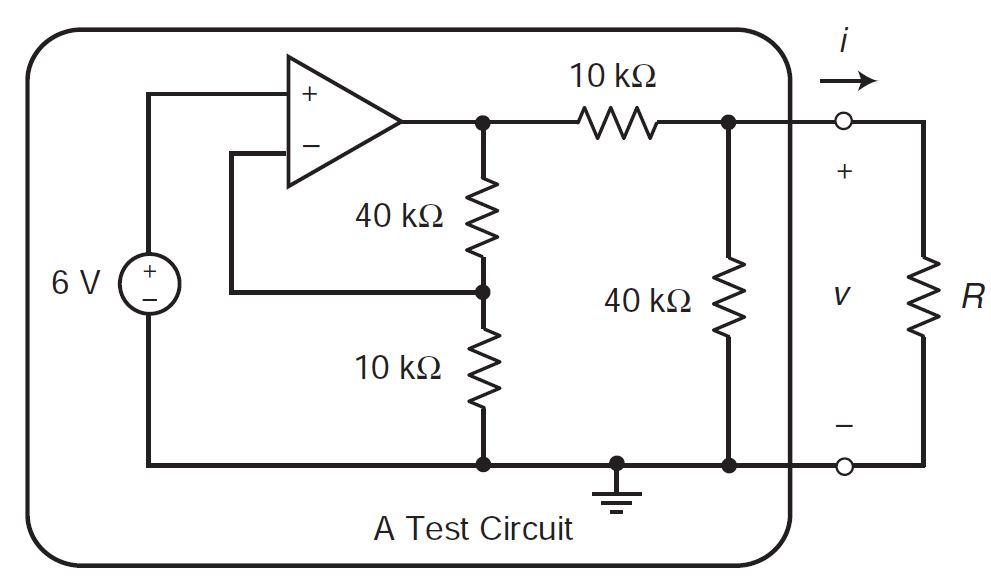
\includegraphics[height=3cm]{figura03.JPG}\\
		%		\end{center}			

		\end{column}
		\begin{column}{0.33\textwidth}  %%<--- here
%\begin{center}
			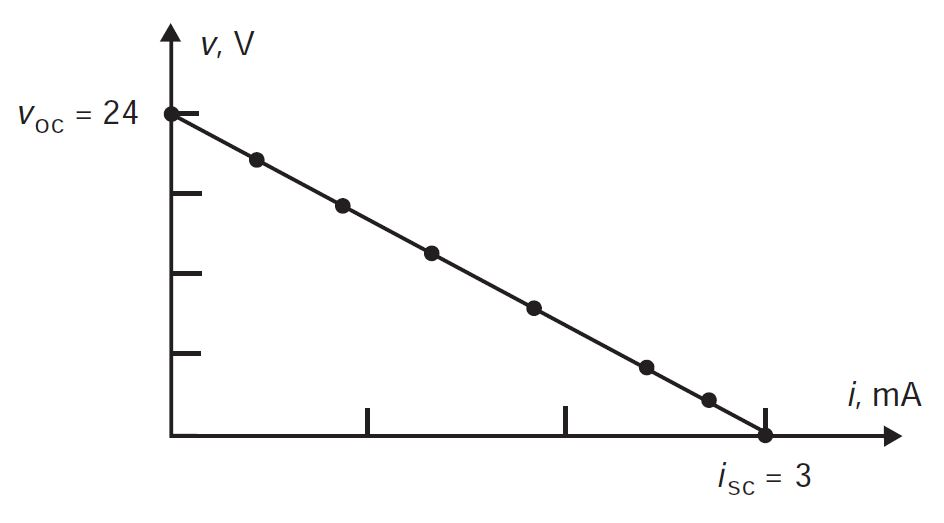
\includegraphics[height=3cm]{figura04.JPG}\\
%	\end{center}	
		\end{column}
	\begin{column}{0.33\textwidth}  %%<--- here
			\begin{equation}
				 v=(-\frac{v_{oc}}{i_{sc}})i+V_{oc}
			\end{equation}
			\begin{equation}
				 v=-Ri+V_{oc}
			\end{equation}
		\end{column}
	
	\end{columns} \\

	\begin{columns}	\column{1\textwidth}
Next, we change the resistor and measure the new values of the resistor voltage and current.\\
	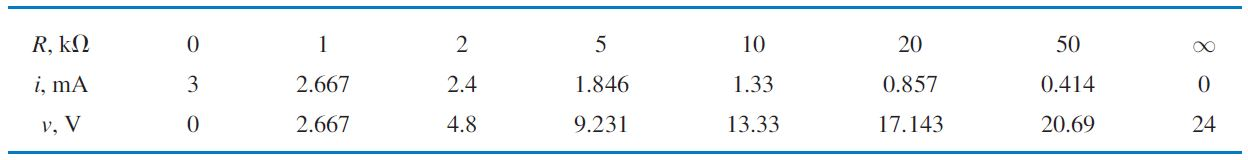
\includegraphics[height=1.7cm]{figura05.JPG}\\
	\end{columns}

\end{tabular}
\end{frame}
% ----------------- NOVO SLIDE --------------------------------
\begin{frame}[fragile]
\frametitle{Source Transformations}
\begin{tabular}{r}
	\begin{columns}	\column{1\textwidth}
	The second and third test circuits have names. They are called the “Thévenin equivalent circuit”
and “Norton equivalent circuit” of the first test circuit. 
\newline
	\end{columns} \\
	\begin{columns}
		\begin{column}{0.4\textwidth}  %%<--- here
		%	\begin{center}

			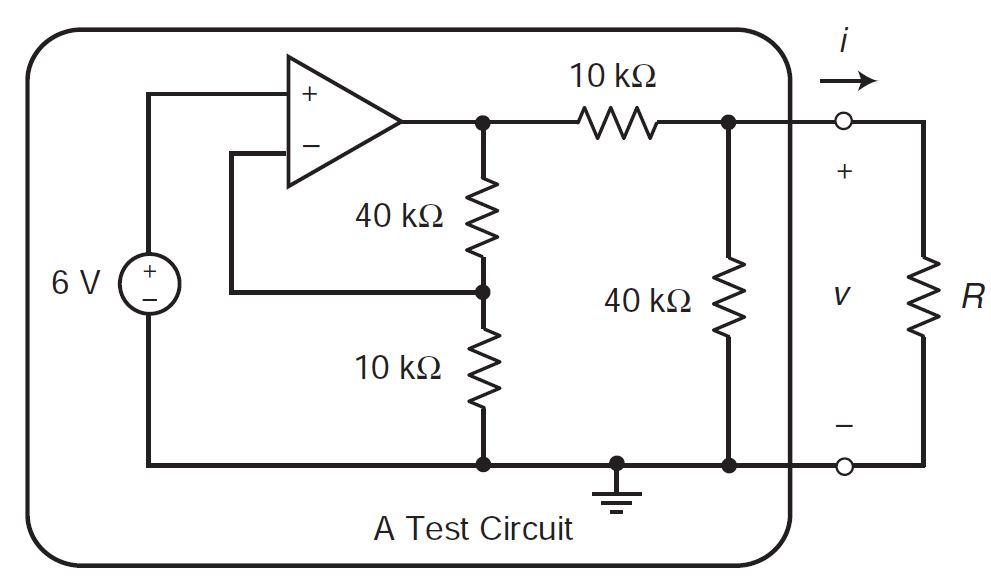
\includegraphics[height=3.2cm]{figura03.JPG}\\


			\begin{equation}
				 v=-Ri+V_{oc}
			\end{equation}
		%		\end{center}			

		\end{column}
		\begin{column}{0.3\textwidth}  %%<--- here
%\begin{center}

			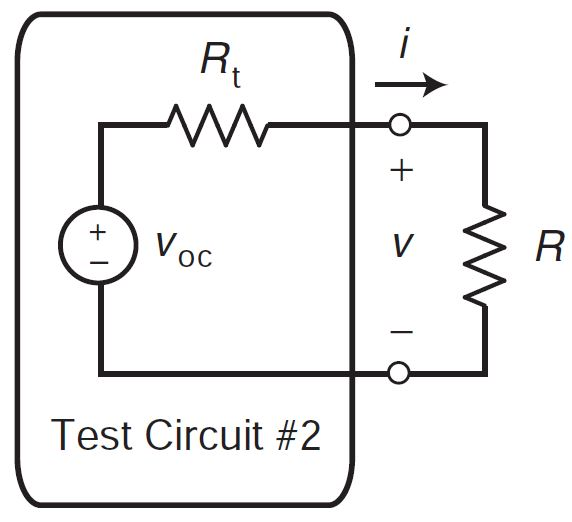
\includegraphics[height=3cm]{figura06.JPG}\\

			\begin{equation}
				 v=-R_{t}i+V_{oc}
			\end{equation}
%	\end{center}	
		\end{column}
	\begin{column}{0.3\textwidth}  %%<--- here
			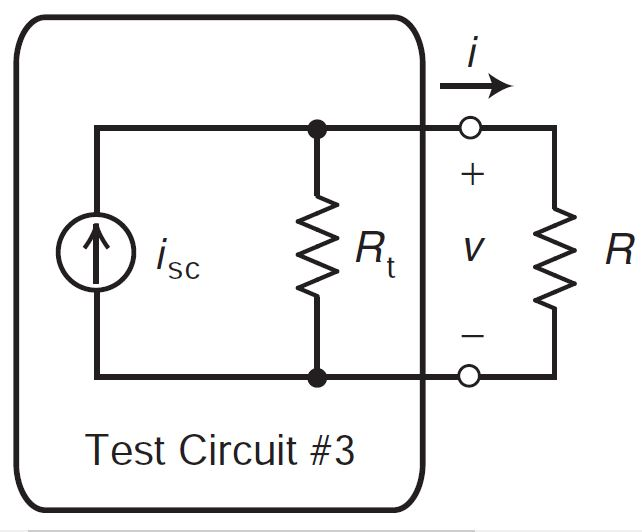
\includegraphics[height=2.9cm]{figura07.JPG}\\

			\begin{equation}
				 v=-R_{t}i+R_{t}i_{sc}
			\end{equation}
		\end{column}
	
	\end{columns} \\


\end{tabular}
\end{frame}
% ----------------- NOVO SLIDE --------------------------------
\begin{frame}[fragile]
\frametitle{Source Transformations}
\begin{tabular}{r}
	\begin{columns}	\column{1\textwidth}
	The second and third test circuits have names. They are called the “Thévenin equivalent circuit”
and “Norton equivalent circuit” of the first test circuit. 
\newline
	\end{columns} \\
	\begin{columns}
		\begin{column}{0.3\textwidth}  %%<--- here
		%	\begin{center}

			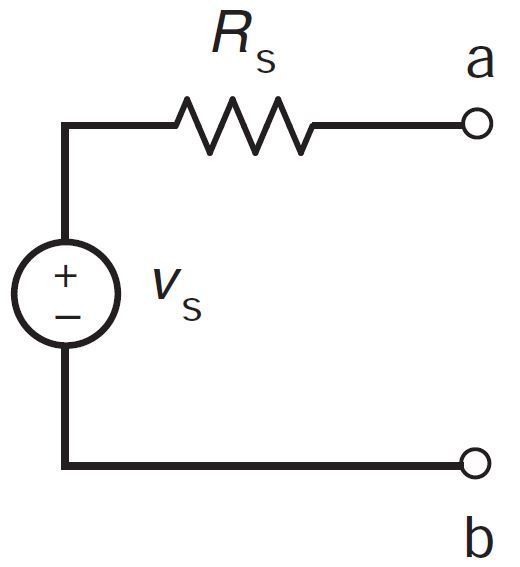
\includegraphics[height=3cm]{figura09.JPG}\\


			\begin{equation}
				 v=-R_{s}i+v_{s}
			\end{equation}
		%		\end{center}			

		\end{column}
		\begin{column}{0.4\textwidth}  %%<--- here
%\begin{center}
	\begin{center}
			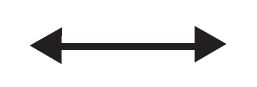
\includegraphics[height=1cm]{figura10.JPG}\\
\end{center}
			\begin{equation}
				 v_{s}=R_{p}i_{p} \ and \ R_{s}=R_{p}
			\end{equation}
			\begin{equation}
				 i_{p}=\frac{V_{s}}{R_{s}} \ and \ R_{p}=R_{s}
			\end{equation}
%	\end{center}	
		\end{column}
	\begin{column}{0.3\textwidth}  %%<--- here
			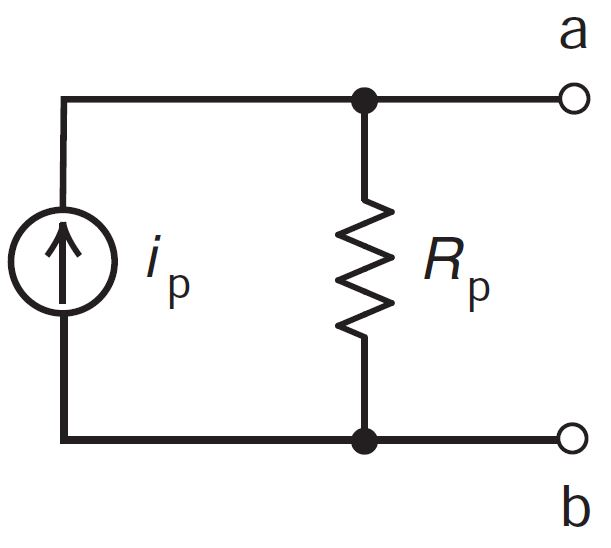
\includegraphics[height=3cm]{figura08.JPG}\\

			\begin{equation}
				 v=-R_{p}i+R_{p}i_{p}
			\end{equation}
		\end{column}
	
	\end{columns} \\


\end{tabular}
\end{frame}

% ----------------- NOVO SLIDE --------------------------------
\begin{frame}[fragile]

	\frametitle{Source Transformations}
\begin{tabular}{ll}
	\begin{columns}
		\begin{column}{1\textwidth}  %%<--- here
		\textbf{EXAMPLE 5.2-2} - First, determine the values of $i_{p}$ and $R_{p}$ that cause the part of the circuit connected to the 2-kV resistor. Next, determine the values of $v_{a}$ and $v_{b}$.\\
		\begin{center}
    			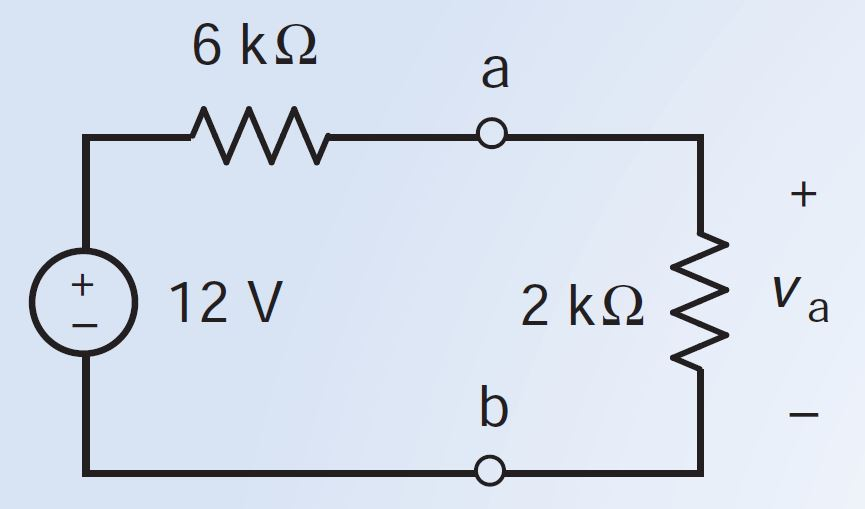
\includegraphics[height=.2\textwidth]{figura12.JPG}	 {             }
			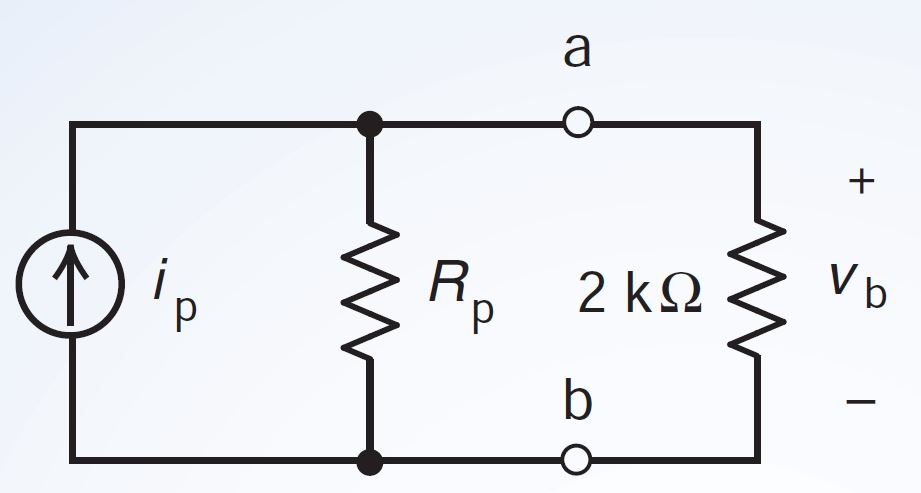
\includegraphics[height=.2\textwidth]{figura13.JPG}	
		\end{center}	
		\scalebox{0.8}{Answer: $R_{p}= 6k\Omega, i_{p}=2mA, v_{a}=3V \ and \ v_{b}=3V$}
		\end{column}
	\end{columns}
\end{tabular}
\end{frame}
% ----------------- NOVO SLIDE --------------------------------
\begin{frame}[fragile]

	\frametitle{Source Transformations}
\begin{tabular}{ll}
	\begin{columns}
		\begin{column}{1\textwidth}  %%<--- here
		\textbf{EXAMPLE 5.2-3} - Use a source transformation to determine a relationship between the resistance $R$ and the resistor current $i$.\\
		\begin{center}
    			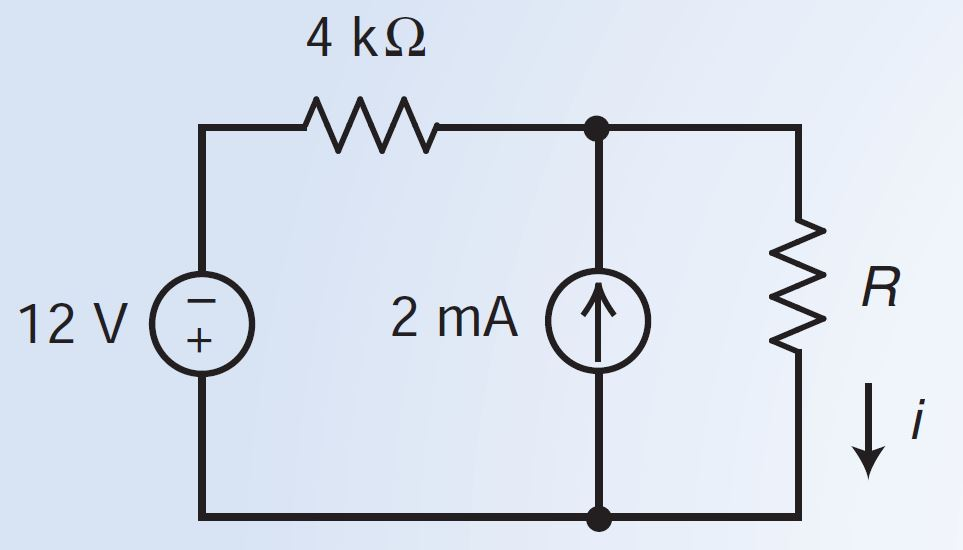
\includegraphics[height=.25\textwidth]{figura11.JPG}	
		
		\end{center}	
		\scalebox{0.8}{Answer: $i=-\frac{4}{4000+R}$}
		\end{column}
	\end{columns}
\end{tabular}
\end{frame}
% ----------------- NOVA SECÇÂO -----------------------------
\section{Superposition (5.3)}
% ----------------- NOVO SLIDE --------------------------------
\begin{frame}[fragile]
\frametitle{Superposition}
		\begin{tabular}{cc}
			\begin{columns}
				\begin{column}{1\textwidth}  %%<--- here
					The output of a linear circuit can be expressed as a linear combination of its inputs. For example,
consider any circuit having the following three properties:	
		
					\begin{itemize}
						\item[$\clubsuit$]{The circuit consists entirely of resistors and dependent and independent sources.}
						\item[$\clubsuit$] {The circuit inputs are the voltages of all the independent voltage sources and the currents of all the
independent current sources.}	
						\item[$\clubsuit$]{The output is the voltage or current of any element of the circuit.}	
		
					\end{itemize}
					
				\end{column}

			\end{columns} \\
			\begin{columns}
				\begin{column}{1\textwidth}  %%<--- here
	{\newline  Consequently, $v_{o}=a_{1}v_{1}+a_{2}v_{2}+a_{3}v_{3}+...+a_{n}v_{n}$,
 where $v_{0}$ is the output of the circuit and $v_{1}, v_{2},..., v_{n}$ are the
inputs to the circuit. The coefficients $a_{1}, a_{2},..., a_{n}$ of the linear combination are real constants called gains.}		
				\end{column}

			\end{columns}




\end{tabular}




\end{frame}

% ----------------- NOVO SLIDE --------------------------------

\begin{frame}[fragile]
\frametitle{Superposition}

\begin{tabular}{r}
	\begin{columns}	\column{1\textwidth}
\textbf{EXAMPLE 5.3-1} - The circuit shown has one output, $v_{o}$, and three inputs, $ v_{1},  i_{2}, \ and \ v_{3}$. 			Express the output as a linear combination of the inputs.
	\end{columns}\\

	\begin{columns}
		\begin{column}{.5\textwidth}  %%<--- here
		
		\begin{center}
    			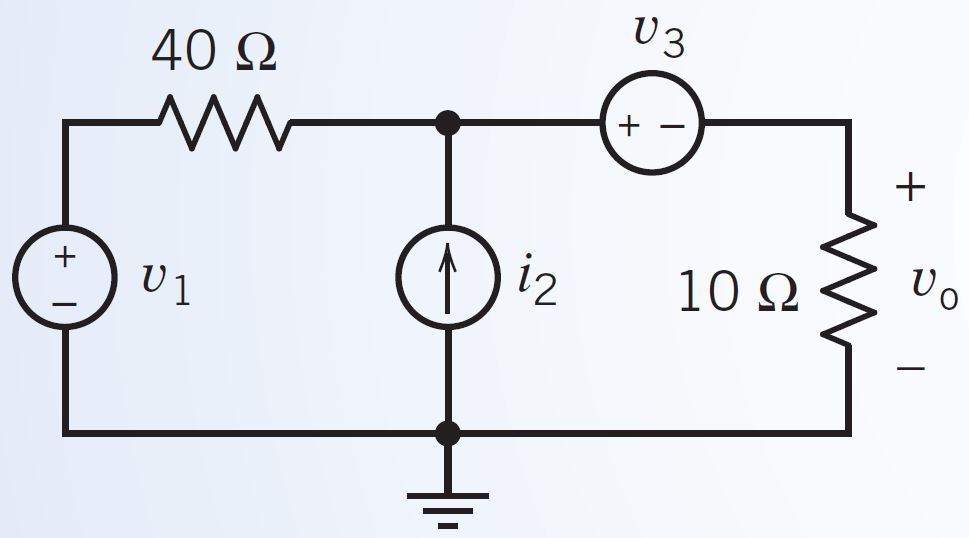
\includegraphics[height=.45\textwidth]{figura14.JPG}	
		
		\end{center}	

		\end{column}

	\begin{column}{.5\textwidth}  %%<--- here
		Because 0-V voltage sources are equivalent to short
		circuits and 0-A current sources are equivalent to open circuits, we replace the sources
		corresponding to the other inputs by short or open circuits. 
		\end{column}




	\end{columns}\\

	\begin{columns}	\column{1\textwidth}
\newline \scalebox{0.8}{Answer: $v_{o}=\frac{v_{1}}{5}+8i_{2}-\frac{v_{3}}{5}$}
	\end{columns}\\

\end{tabular}

\end{frame}
% ----------------- NOVO SLIDE --------------------------------
\begin{frame}[fragile]

	\frametitle{Superposition}
\begin{tabular}{ll}
	\begin{columns}
		\begin{column}{.5\textwidth}  %%<--- here
		\textbf{EXAMPLE 5.3-2} - Find the current i for the circuit.\\
		\begin{center}
    			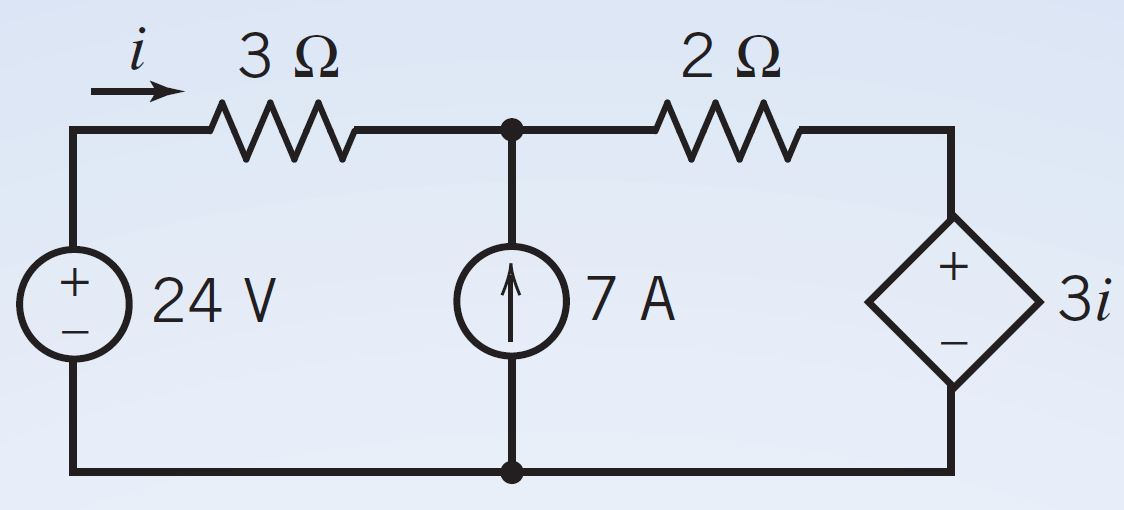
\includegraphics[height=.45\textwidth]{figura15.JPG}	
		
		\end{center}	
		\scalebox{0.8}{Answer: $i=\frac{5}{4}$}
		\end{column}
				\begin{column}{.5\textwidth}  %%<--- here
The output of a linear circuit due to several inputs working together is equal to the sum of the
outputs due to each input working separately.
				\end{column}
		
		
		
		
		
		
	\end{columns}
\end{tabular}
\end{frame}

% ----------------- NOVA SECÇÂO -----------------------------
\section{Thévenin's Theorem (5.4)}
% ----------------- NOVO SLIDE --------------------------------
\begin{frame}[fragile]
\frametitle{Thévenin's Theorem}
\begin{tabular}{r}
	\begin{columns}	\column{1\textwidth}
In this section, we introduce the Thévenin equivalent circuit, based on a theorem developed by M. L.
Thévenin, a French engineer, who first published the principle in 1883.
	\end{columns}\\

	\begin{columns}
		\begin{column}{.4\textwidth}  %%<--- here
		
		\begin{center}
    			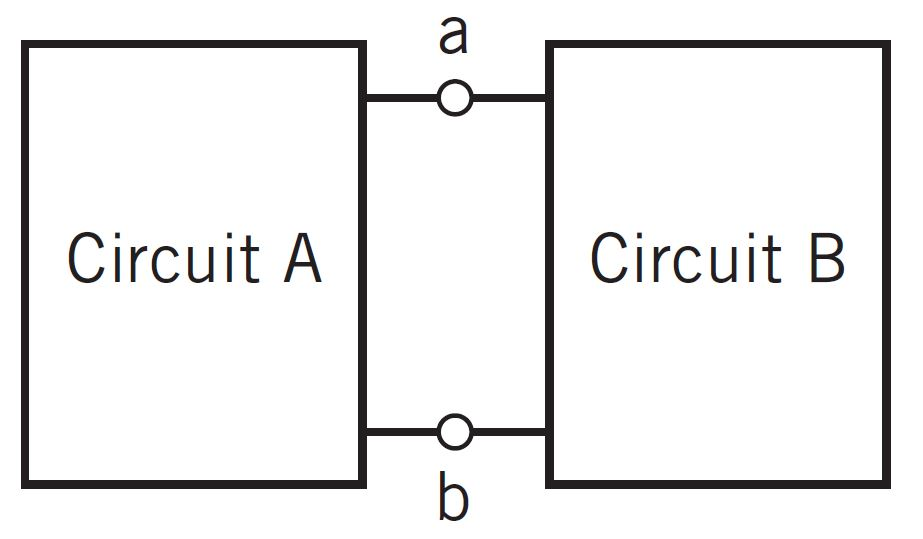
\includegraphics[height=.4\textwidth]{figura16.JPG}\\	
			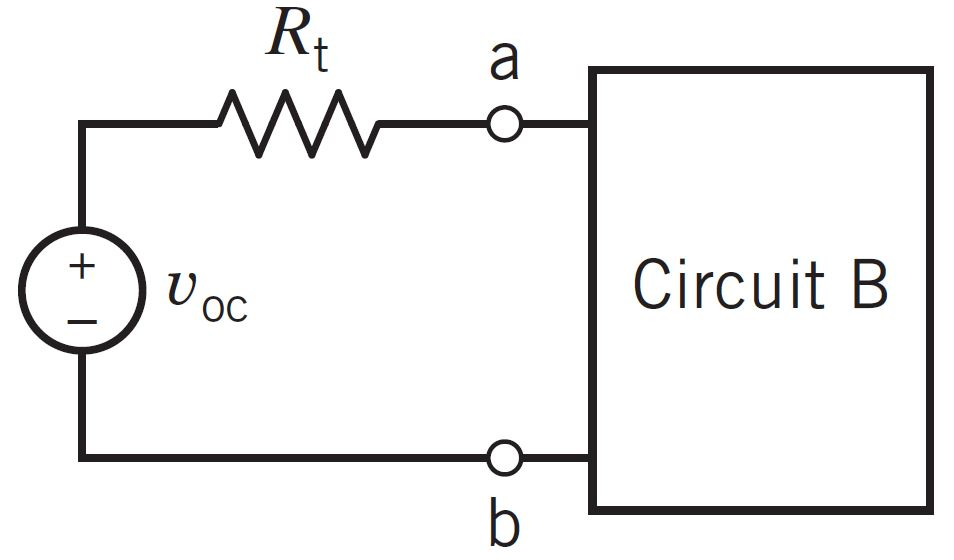
\includegraphics[height=.4\textwidth]{figura17.JPG}	
		
		\end{center}	

		\end{column}
	\begin{column}{.6\textwidth}  %%<--- here

Finding the Thévenin equivalent circuit of circuit "A" involves three parameters: \newline
			\begin{itemize}
			\item[$\clubsuit$]{The open-circuit voltage, $v_{oc}$.}
			\item[$\clubsuit$] {The short-circuit current, $i_{sc}$.}	
			\item[$\clubsuit$]{Thévenin resistance, $R_{t}$.}	
		
			\end{itemize}


	\end{column}

	\end{columns}

\end{tabular}

\end{frame}
% ----------------- NOVO SLIDE --------------------------------
\begin{frame}[fragile]
\frametitle{Thévenin's Theorem}
\begin{tabular}{r}
	\begin{columns} \column{1\textwidth}
Finding the Thévenin equivalent circuit of circuit "A" involves three parameters: 
	\end{columns}\\

	\begin{columns}
		
	\begin{column}{.45\textwidth}  %%<--- here


			\begin{itemize}
			\item[$\clubsuit$]{The open-circuit voltage, $v_{oc}$.\newline }
			\item[$\clubsuit$] {The short-circuit current, $i_{sc}$.\newline }	
			\item[$\clubsuit$]{Thévenin resistance, $R_{t}$.}	
		
			\end{itemize}


	\end{column}
\begin{column}{.5\textwidth}  %%<--- here
		
		\begin{center}
    			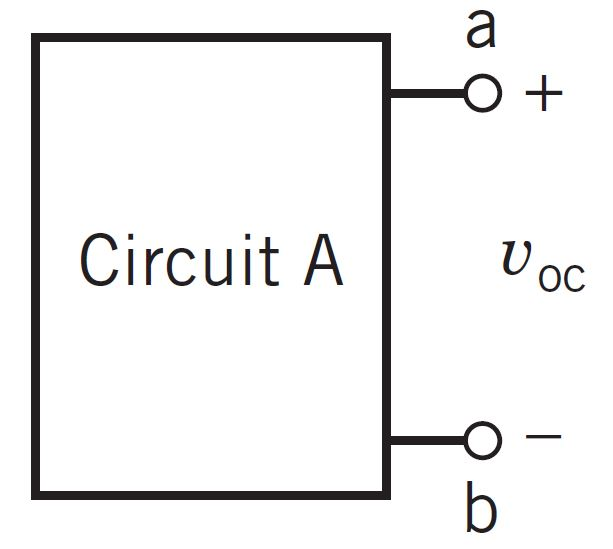
\includegraphics[height=.3\textwidth]{figura18.JPG}	{}
			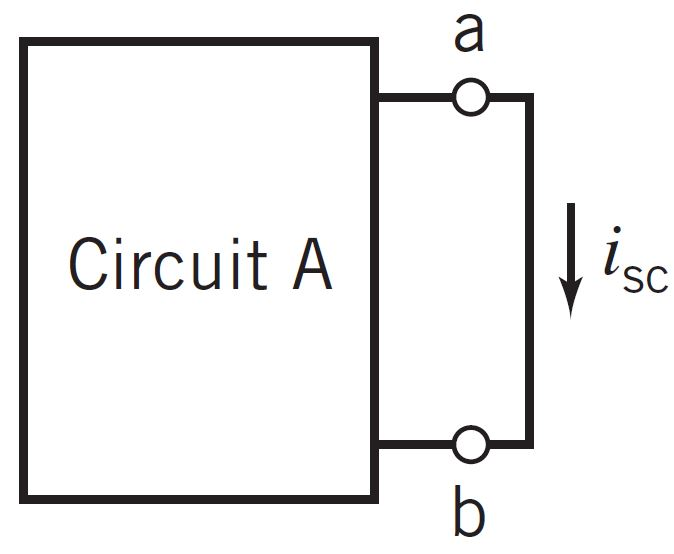
\includegraphics[height=.3\textwidth]{figura19.JPG}	{}
			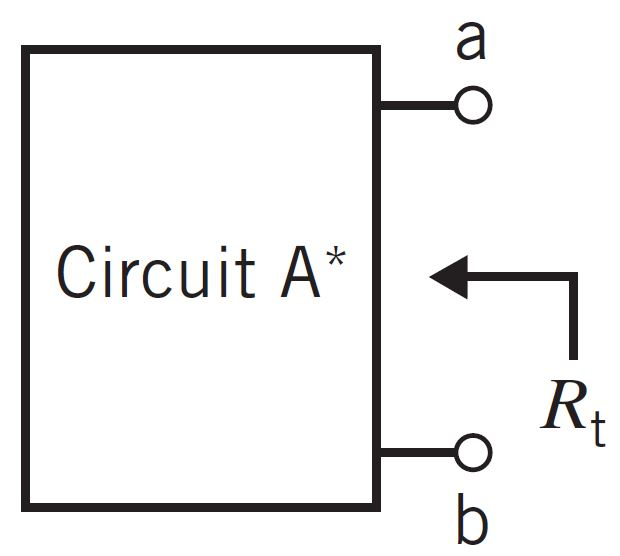
\includegraphics[height=.3\textwidth]{figura20.JPG}
		 
		\end{center}	

		\end{column}

	\end{columns}

\end{tabular}

\end{frame}
% ----------------- NOVO SLIDE --------------------------------
\begin{frame}[fragile]

	\frametitle{Thévenin's Theorem}
\begin{tabular}{ll}
	\begin{columns}
		\begin{column}{1\textwidth}  %%<--- here
		\textbf{EXAMPLE 5.4-1} - Determine the Thevenin equivalent circuit for the circuit shown.\\
		\begin{center}
    			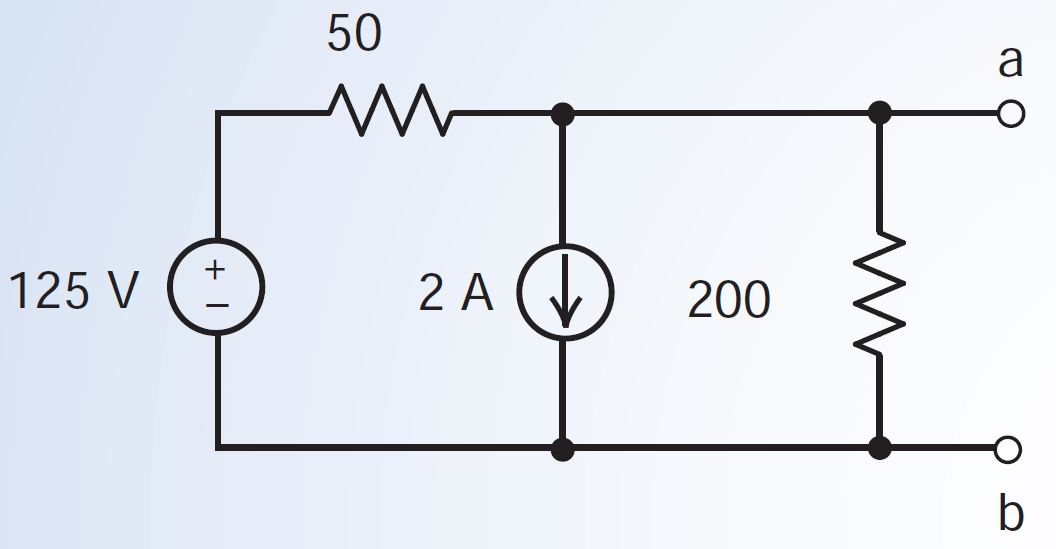
\includegraphics[height=.25\textwidth]{figura21.JPG}	
		
		\end{center}	
		\scalebox{0.8}{Answer: $v_{oc}=20V, I_{sc}=0.5A \ and \ R_{t}=40\Omega$}
		\end{column}
	\end{columns}
\end{tabular}
\end{frame}
% ----------------- NOVO SLIDE --------------------------------
\begin{frame}[fragile]

	\frametitle{Thévenin's Theorem Circuit of a Circuit
Containing a Dependent Source}
\begin{tabular}{ll}
	\begin{columns}
		\begin{column}{1\textwidth}  %%<--- here
		\textbf{EXAMPLE 5.4-2} - Determine the Thevenin equivalent circuit for the circuit shown.\\
		\begin{center}
    			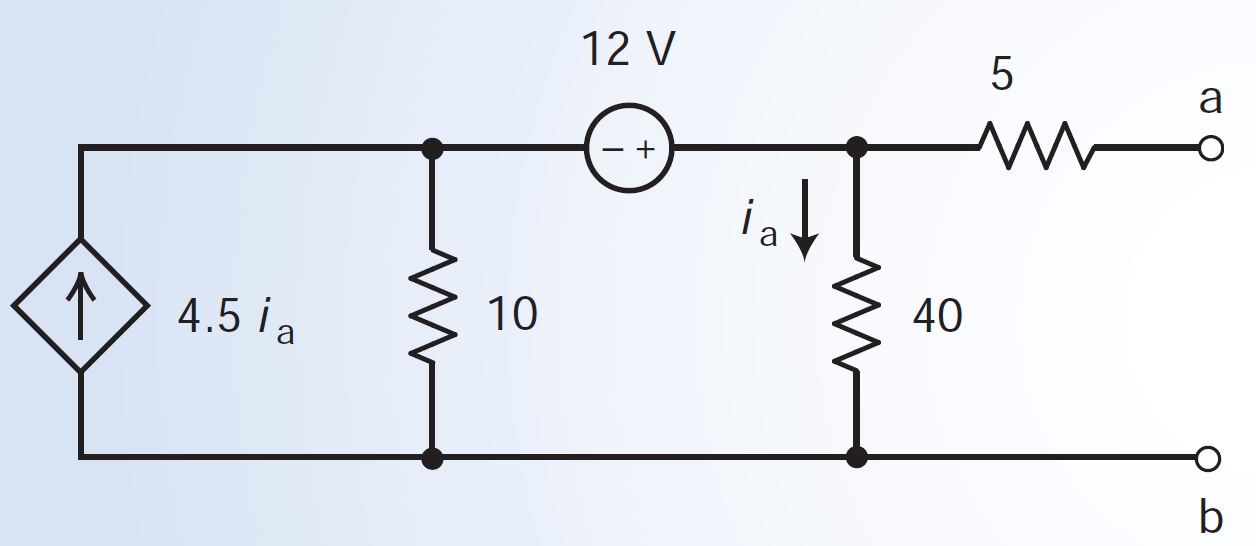
\includegraphics[height=.25\textwidth]{figura22.JPG}	
		
		\end{center}	
		\scalebox{0.8}{Answer: $v_{oc}=96V, I_{sc}=1.1294A \ and \ R_{t}=85\Omega$}
		\end{column}
	\end{columns}
\end{tabular}
\end{frame}
% ----------------- NOVA SECÇÂO -----------------------------
\section{Norton's Equivalent Circuit (5.5)}
% ----------------- NOVO SLIDE --------------------------------
\begin{frame}[fragile]
  \frametitle{Norton's Theorem}
\begin{tabular}{r}
	\begin{columns}	\column{1\textwidth}
E. L. Norton, proposed an equivalent circuit using a current source and an equivalent resistance.
	\end{columns}\\

	\begin{columns}
		\begin{column}{.4\textwidth}  %%<--- here
		
		\begin{center}
    			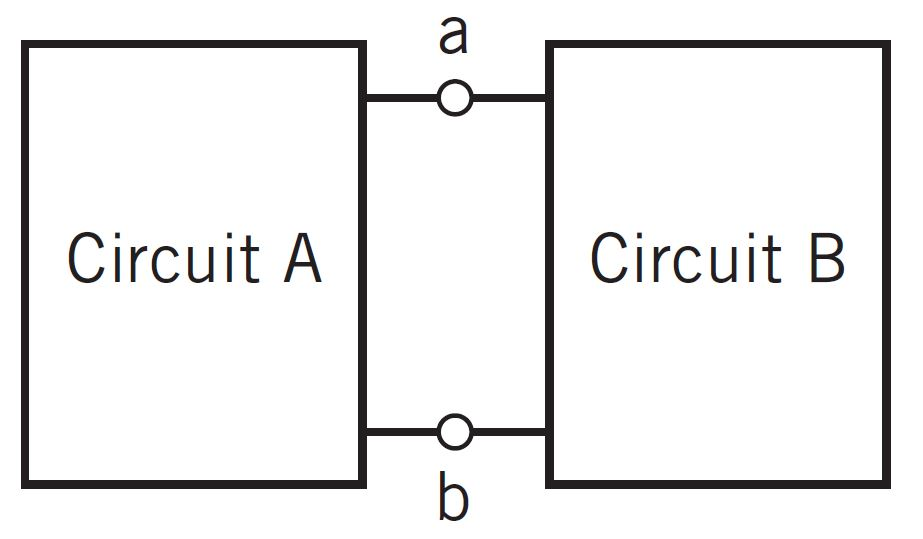
\includegraphics[height=.4\textwidth]{figura16.JPG}\\	
			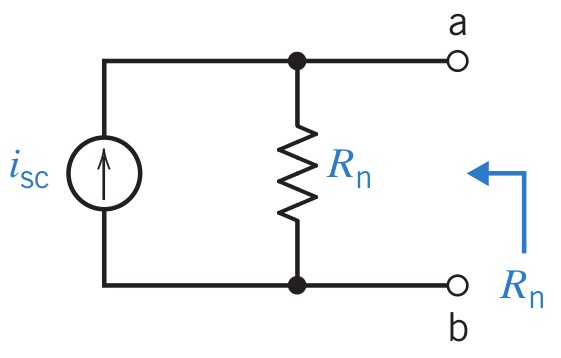
\includegraphics[height=.4\textwidth]{figura23.jpg}	
		
		\end{center}	

		\end{column}
	\begin{column}{.6\textwidth}  %%<--- here

Finding the Norton equivalent circuit of circuit "A" involves two parameters: \newline
			\begin{itemize}
			\item[$\clubsuit$] {The short-circuit current, $i_{sc}$.}	
			\item[$\clubsuit$]{Norton resistance, $R_{n}$.}	
		
			\end{itemize}
		    \begin{center}
		     The Norton equivalent is simply the source transformation of the Thévenin
equivalent ($R_{n}=R_{t} \ and \ v_{oc}=R_{t}i_{sc} $).

		    \end{center}


	\end{column}

	\end{columns}

\end{tabular}
\end{frame}

% ----------------- NOVO SLIDE --------------------------------

\begin{frame}[fragile]
  \frametitle{Norton's Theorem}
\begin{tabular}{ll}
	\begin{columns}
		\begin{column}{1\textwidth}  %%<--- here
		\textbf{EXAMPLE 5.5-1} - Determine the Norton equivalent circuit for the circuit shown.\\
		\begin{center}
    			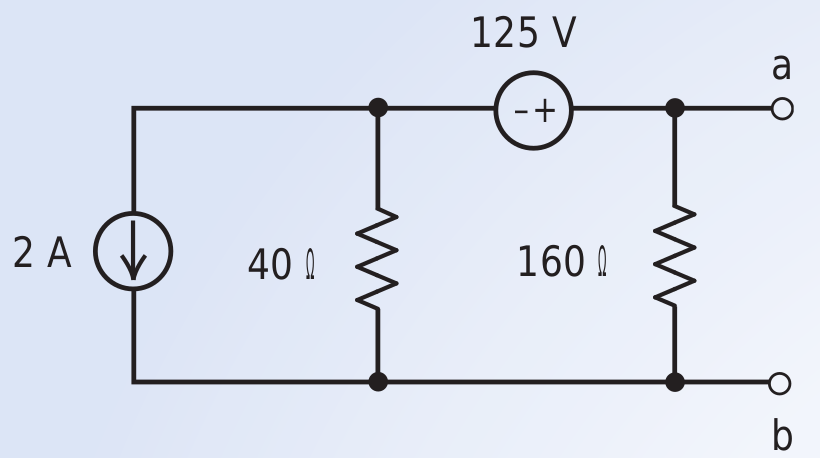
\includegraphics[height=.25\textwidth]{figura24.jpg}	
		
		\end{center}	
		\scalebox{0.8}{Answer: $i_{sc}=1.125A \ and \ R_{n}=32\Omega$}
		\end{column}
	\end{columns}
\end{tabular}
\end{frame}

% ----------------- NOVO SLIDE --------------------------------

\begin{frame}[fragile]
  \frametitle{Norton Equivalent Circuit of a Circuit
Containing a Dependent Source}
\begin{tabular}{ll}
	\begin{columns}
		\begin{column}{1\textwidth}  %%<--- here
		\textbf{EXAMPLE 5.5-2} - Determine the Norton equivalent circuit for the circuit shown.\\
		\begin{center}
    			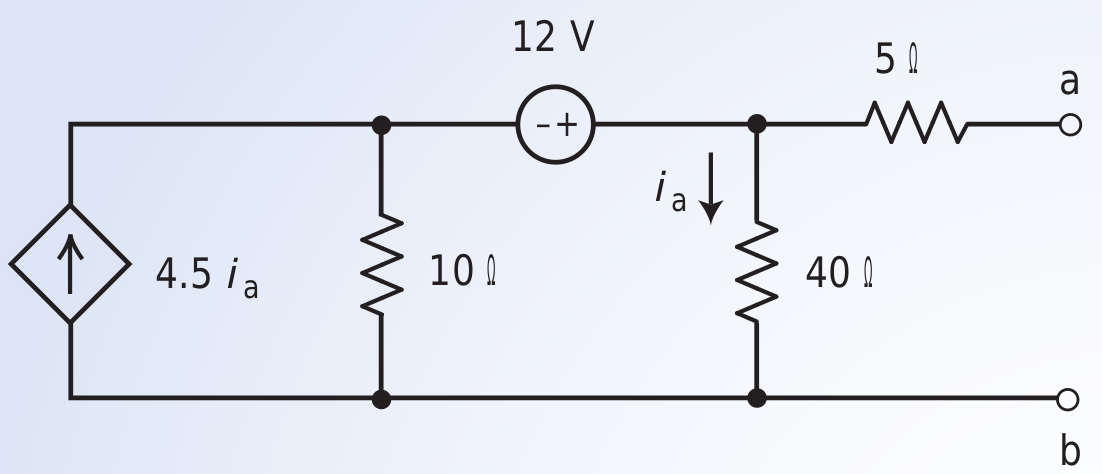
\includegraphics[height=.25\textwidth]{figura25.png}	
		
		\end{center}	
		\scalebox{0.8}{Answer: $v_{oc}=96, i_{sc}=1.13A \ and \ R_{t}=85\Omega$}
		\end{column}
	\end{columns}
\end{tabular}
\end{frame}
% ----------------- NOVO SLIDE --------------------------------

\begin{frame}[fragile]
  \frametitle{Norton Equivalent Circuit of a Circuit
Containing a Dependent Source}
\begin{tabular}{ll}
	\begin{columns}
		\begin{column}{1\textwidth}  %%<--- here
		\textbf{EXERCISE 5.5-1} - Determine values of $R_{t}$ and $i_{sc}$ that cause the circuit shown in Figure
a to be the Norton equivalent circuit of the circuit in Figure b.\\
		\begin{center}
    			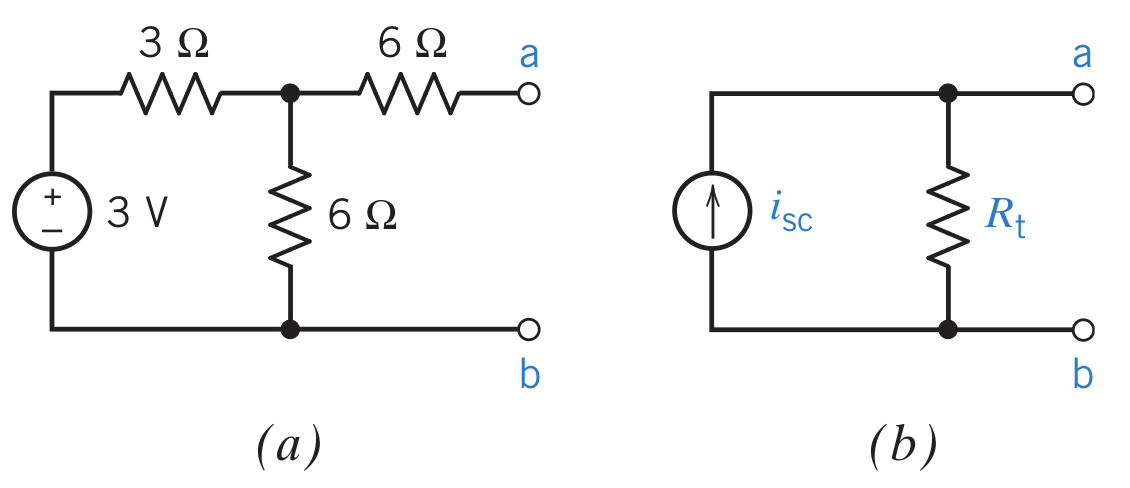
\includegraphics[height=.25\textwidth]{figura26.png}	
		
		\end{center}	
		\scalebox{0.8}{Answer: $i_{sc}=0.25A \ and \ R_{t}=8\Omega$}
		\end{column}
	\end{columns}
\end{tabular}
\end{frame}
% ----------------- NOVA SECÇÂO -----------------------------
\section{Maximum Power Transfer (5.6)}
% ----------------- NOVO SLIDE --------------------------------
\begin{frame}[fragile]
\frametitle{Maximum Power Transfer}
\begin{tabular}{r}
	\begin{columns}	\column{1\textwidth}
	Many applications of circuits require the maximum power available from a source to be transferred to a load
resistor $R_{L}$.
\newline
	\end{columns} \\
	\begin{columns}
		\begin{column}{.2\textwidth}  %%<--- here
	%		\begin{center}
			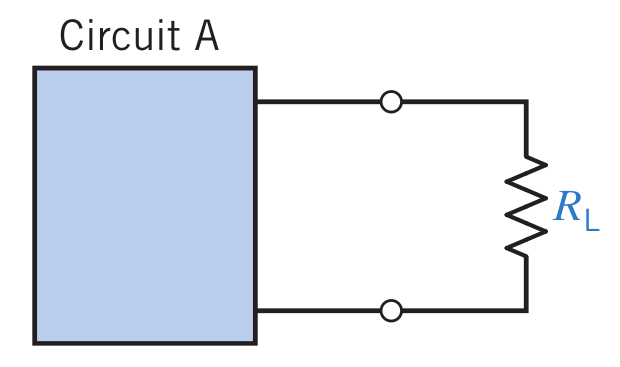
\includegraphics[height=3cm]{figura27.png}\\
	%		\end{center}			

		\end{column}
		\begin{column}{0.4\textwidth}  %%<--- here
			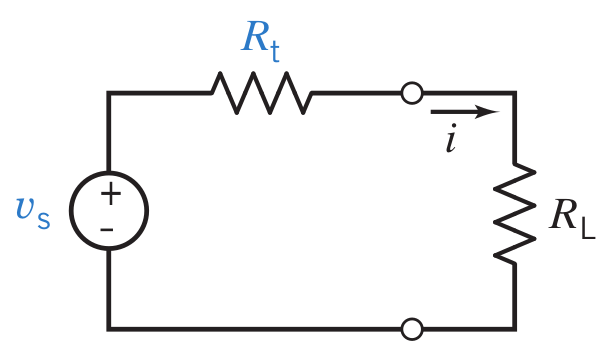
\includegraphics[height=3cm]{figura28.png}\\
		\end{column}
	\end{columns} \\

	\begin{columns}	\column{1\textwidth}
	\newline The general problem of power transfer can be discussed in terms of efficiency and effectiveness.
Power utility systems are designed to transport the power to the load with the greatest efficiency by
reducing the losses on the power lines.
	\end{columns}

\end{tabular}
\end{frame}


% ----------------- NOVO SLIDE --------------------------------
\begin{frame}[fragile]
\frametitle{Maximum Power Transfer}
\begin{tabular}{r}
	\begin{columns}	\column{1\textwidth}
	Let us consider the general circuit of Figure.
\newline
	\end{columns} \\
	\begin{columns}
		\begin{column}{0.3\textwidth}  %%<--- here
	%		\begin{center}
			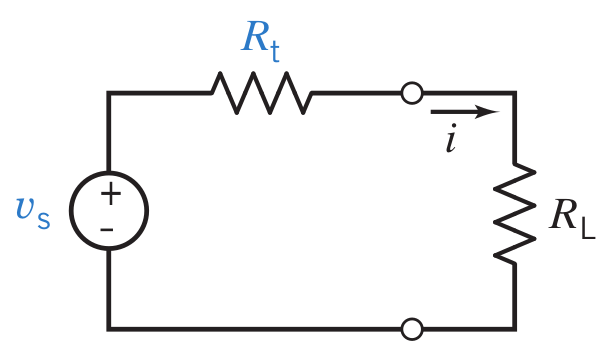
\includegraphics[height=3cm]{figura28.png}\\
			%	\end{center}			

		\end{column}
		\begin{column}{0.7\textwidth}  %%<--- here
			\begin{equation}
				 p=i^{2}R_{L}, i=\frac{v_{s}}{R_{L}+R_{t}} \ and \ p=(\frac{v_{s}}{R_{L}+R_{t}})^{2}R_{L}
			\end{equation}			
			\begin{equation}
				 \frac{dp}{dR_{L}}=v_{s}^{2}\frac{(R_{t}+R_{L})^{2}-2(R_{t}+R_{L})R_{L}}{(R_{L}+R_{t})^{4}}
			\end{equation}
			
			\begin{equation}
				 (R_{t}+R_{L})^{2}-2(R_{t}+R_{L})R_{L}=0
			\end{equation}		
			\begin{equation}
				 (R_{t}+R_{L})(R_{t}+R_{L}-2R_{L})=0
			\end{equation}
			\begin{equation}
				Solving\ (13), we\ obtain\ R_{t}=R_{L}.
			\end{equation}
			\end{column}
	
	\end{columns} \\

	

\end{tabular}
\end{frame}


% ----------------- NOVO SLIDE --------------------------------
\begin{frame}[fragile]
\frametitle{Maximum Power Transfer}
\begin{tabular}{r}
	
	\begin{columns}
		\begin{column}{0.4\textwidth}  %%<--- here
	%		\begin{center}
			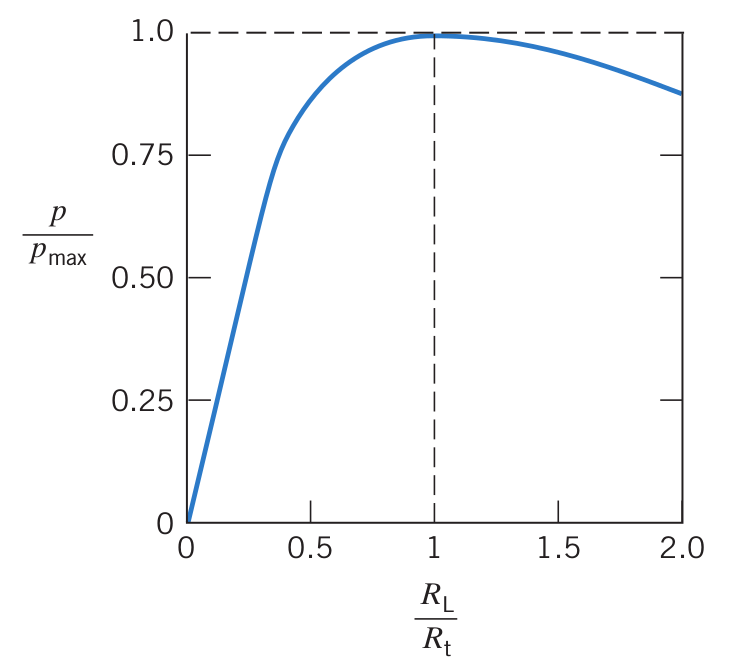
\includegraphics[height=5cm]{figura29.png}\\
			%	\end{center}			

		\end{column}
		\begin{column}{0.6\textwidth}  %%<--- here
			The \textbf{maximum power transfer} theorem states that the maximum power delivered to a load by
a source is attained when the load resistance, $R_{L}$ , is equal to the Thévenin resistance, $R_{t}$, of the
source.
\newline
			\begin{equation}
				 p_{max}=\frac{v_{s}^{2}R_{t}}{(2R_{t})^{2}}=\frac{v_{s}^{2}}{(4R_{t})}
			\end{equation}			
		\end{column}
	
	\end{columns} \\


\end{tabular}
\end{frame}
% ----------------- NOVO SLIDE --------------------------------

\begin{frame}[fragile]
  \frametitle{Maximum Power Transfer}
\begin{tabular}{ll}
	\begin{columns}
		\begin{column}{1\textwidth}  %%<--- here
		\textbf{EXEMPLE 5.6-2} - Find the load $R_{L}$ that will result in maximum power delivered to the load of the circuit. Also,
determine $p_{max}$ delivered.\\
		\begin{center}
    			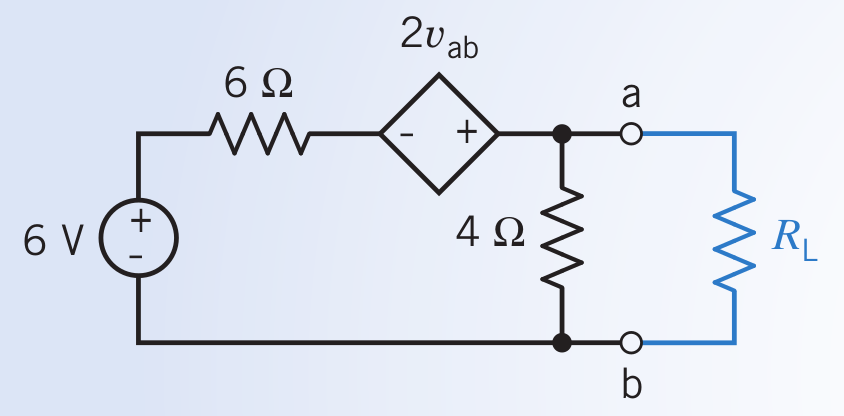
\includegraphics[height=.25\textwidth]{figura30.png}	
		
		\end{center}	
		\scalebox{0.8}{Answer: $R_{L}=R_{t}=12\Omega \ and \ p_{max}=3W$}
		\end{column}
	\end{columns}
\end{tabular}
\end{frame}
% ----------------- NOVO SLIDE --------------------------------

\begin{frame}[fragile]
  \frametitle{Maximum Power Transfer}
\begin{tabular}{ll}
	\begin{columns}
		\begin{column}{1\textwidth}  %%<--- here
		\textbf{EXERCISE 5.6-1} - Find the maximum power that can be delivered to $R_{L}$ for the circuit of Figure, using a Thévenin equivalent circuit.\\
		\begin{center}
    			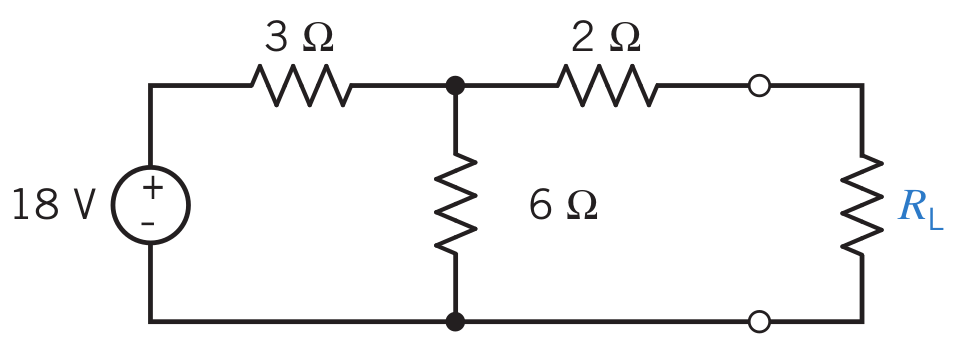
\includegraphics[height=.25\textwidth]{figura31.png}	
		
		\end{center}	
		\scalebox{0.8}{Answer: $9 \ W \ when \ R_{L}=4\Omega$}
		\end{column}
	\end{columns}
\end{tabular}
\end{frame}

% ----------------- NOVA SECÇÂO -----------------------------
\section{Using MATLAB to Determine the Thévenin Equivalent Circuit (5.7)}
% ----------------- NOVO SLIDE --------------------------------
\begin{frame}[fragile]
\frametitle{Using MATLAB to Determine the Thévenin Equivalent Circuit}
\begin{tabular}{r}
	
	\begin{columns}
		\begin{column}{0.4\textwidth}  %%<--- here
	%		\begin{center}
			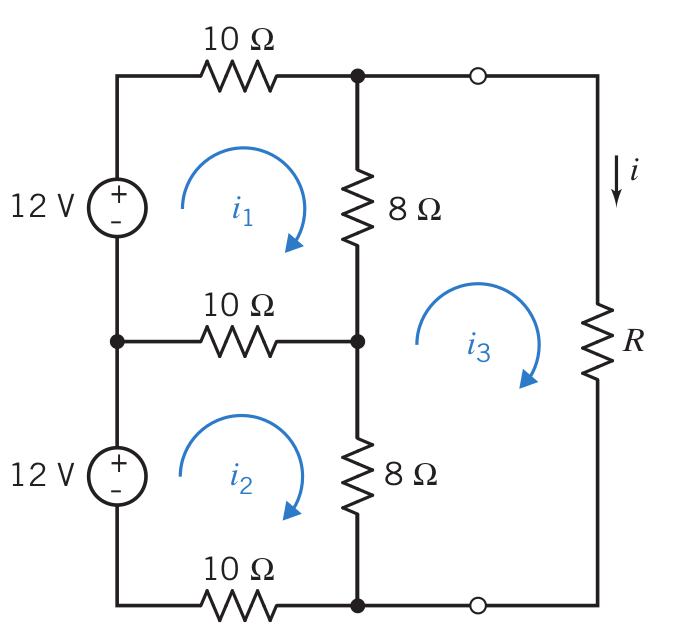
\includegraphics[height=5cm]{figura32.png}\\
			%	\end{center}			

		\end{column}
		\begin{column}{0.6\textwidth}  %%<--- here
			MATLAB can be used to reduce the work required to determine the Thévenin equivalent of a circuit
such as the one shown in Figure.
\newline
				\[ 
			\left[\begin{array}{rrr}
			28 & -10 & -8 \\
			-10 & 28 & -8 \\
			-8 & -8 & 16+R \end{array} \right]
			\left[\begin{array}{c}
			i_{1} \\
			i_{2} \\
			 i_{3}\end{array} \right]= 
			\left[\begin{array}{r}
			12 \\
			12 \\
			0  \end{array} \right]
			\]	
			
			
				\[ 
			\left[\begin{array}{r}
			R_{a}i_{a} \\
			R_{b}i_{b} \end{array} \right]=
			\left[\begin{array}{rr}
			1 & -i_{a} \\
			1 & -i_{b} \end{array} \right]
			\left[\begin{array}{c}
			v_{t} \\
			R_{t}\end{array} \right] 			
			\]	
			
			
			
			
			
		\end{column}
	
	\end{columns} \\


\end{tabular}
\end{frame}
\end{document} 